\section{OOD detection in multi-label setting}
As mentioned previously, research on detecting Out-Of-Distribution in multi-label classifiers has quite recently just begun, 
resulting in a limited number of approaches. 
Most of the methods adopt concepts and ideas from multi-class OOD detection. 
In this section, we will provide a more detailed overview description of state-of-the-art OOD detectors in multi-label setting.

\subsection{JointEnergy detector}
\paragraph{Using energy function and summation}
In 2021, Wang et al.~\cite{Wang2021} introduced JointEnergy, a simple and effective method for estimating OOD indicator scores by aggregating label-wise energy scores from multiple labels. 
In multi-label settings, MaxLogit\cite{hendrycksScalingOutofDistributionDetection2022} served as the baseline for OOD detection. 
MaxLogit obtains logits from the neural network and takes the maximum of these logits as a score. 
JointEnergy introduces two fundamental changes. 
Firstly, it uses energy scores instead of logits, and secondly, it take the sum across the classes instead of maximum. 
Liu, Weitang and Wang~\cite{liuEnergybasedOutofdistributionDetection2021} demonstrated that the energy-based approach can enhance OOD uncertainty estimation for multi-class settings and in this paper, 
it is proven the efficiency for multi-label settings as well. 

Multi-label classifier can be interpreted from energy-based perspective by viewing the logit 
$f_{y_i}(\mathbf{x})$ of class $y_i$ as an energy function $E_{y_i}(\mathbf{x}, y_i) = - f_{y_i}(\mathbf{x})$. 
Without changing the parameterization of the neural network f (x), we can express the free energy function $E_{\text{joint}}(\mathbf{x})$ over $\mathbf{x} \in \mathbb{R}^D$:
The free energy function is computed by aggregating the label-wise energy scores from multiple labels.

\begin{equation}
\centering
E_{y_i}(\mathbf{x}, f) = \log{(1 + e^{f_{y_i}(\mathbf{x})})}
\end{equation}
\begin{equation}
\centering
E_{\text{joint}}(\mathbf{x}) = \sum_{i=1}^{K}{-E_{y_i}(\mathbf{x}, f)}
\end{equation}

Label-wise energy $E_{y_i}(\mathbf{x})$ by definition is a negative value, and the aggregation methods output a positive value by negation. 
This aligns with the convention that a larger score indicates in-distribution and vice versa.

The authors emphasize the importance of both the \textbf{scoring function}, \textbf{aggregation function} as well as \textbf{their compatibility} to achieve an accurate OOD detection. 
They proved that using summation over the labels makes the estimation much stronger than just taking the maximum. This can be seen in \autoref{fig:energy}

\begin{figure}[h!]
\centering
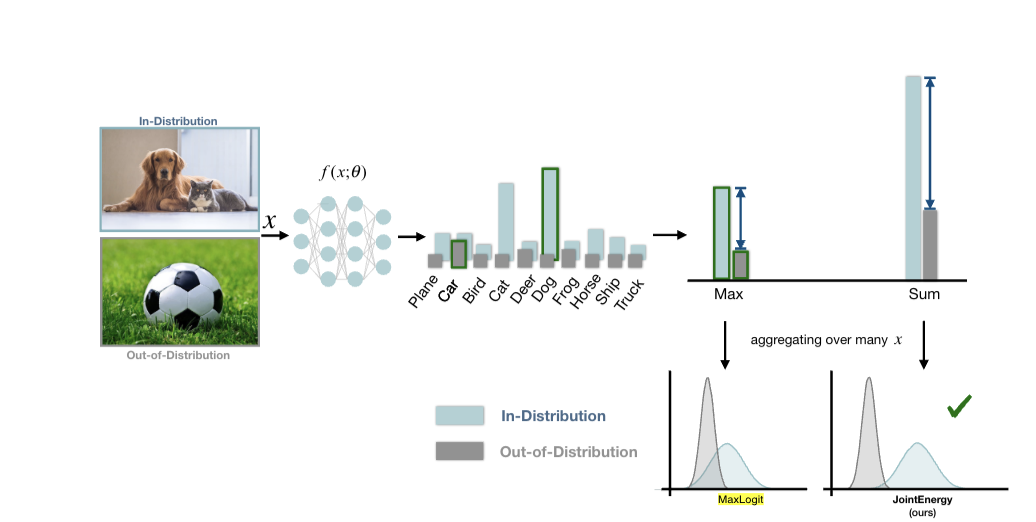
\includegraphics[width=\linewidth]{fig/energy_aggregation.png}
\caption{OOD scores are either the maximum-valued score (denoted by green outlines) or the sum of all scores. 
Taking the sum results in a larger difference in scores and more separation between in-distribution and OOD inputs (denoted by red lines),
resulting in better OOD detection. 
Plots in the bottom right depict the probability densities of MaxLogit\cite{hendrycksScalingOutofDistributionDetection2022} versus JointEnergy\cite{Wang2021}}
\label{fig:energy}
\end{figure}


\subsection{YolOOD}
\paragraph{Using object detector}
In 2022, Zolfi et al. presented YolOOD~\cite{Zolfi2022}, a novel method for out-of-distribution (OOD) detection in the multi-label classification task. 
The main contribution of this paper is the utilization of concepts from object detection to perform OOD detection. 
The authors convert a regular object detection model Yolo~\cite{bochkovskiyYOLOv4OptimalSpeed2020} into an image classifier with inherent OOD detection capabilities with just minor changes.
Object detectors have an inherent ability to distinguish between objects of interest (in-distribution data) and irrelevant objects (OOD data) making them perfect candidates
for fulfilling the goals of the OOD detection task. Yolo object detector predicts objectness score and probability class scores for every cell in the grid.

\paragraph{Network architecture}
Yolo has a backbone network and three detection heads that process features at different scales.
YolOOD has an adapted last layer of the detector to produce the image-wise scores and objectness scores. An overview of the network's pipeline can be seen in \autoref{fig:yolo}.

\paragraph{Yolo Objectness score}
The training of object detectors involves passive negative learning, where unlabeled data in training images helps the model discard irrelevant objects. YOLO uses objectness scores to achieve this. 
The YOLO objectness score is a single value that represents the model's confidence that the bounding box contains an object. 
In YolOOD, the objectness score is used as one of the components of the custom loss function devised to train the model. 
The objectness score for a candidate (cell in the grid) $c$ is:
\begin{equation}
\centering
c_{\text{obj}}(i,j) =
\left\{
    \begin{array}{ll}
        1  & \mbox{if } \varphi_u \wedge \varphi_s \wedge \varphi_l \wedge \varphi_r \\
        0  & \mbox{if } \text{otherwise}
    \end{array}
\right.
\end{equation}

\begin{equation}
\centering
\begin{aligned}
\varphi_u = i \geq x_{\text{center}} - p * \frac{W'}{2}, \varphi_l = j \geq y_{\text{center}} - p * \frac{H'}{2} \\
\varphi_d = i \leq x_{\text{center}} + p * \frac{W'}{2}, \varphi_r = j \leq y_{\text{center}} + p * \frac{H'}{2}
\end{aligned}
\end{equation}

where $W (H)$ is the width (height) of the image respectively and $p$ is the portion of grid cells relative to the grid’s size, with regard to the object’s center.

\paragraph{Class score}
Class score for a class $n \in {1, \dots , N_c}$ in a specific candidate (cell in the grid) $c$ is:
\begin{equation}
\centering
c_{\text{cls n}} =
\left\{
    \begin{array}{ll}
        1  & \mbox{if } \text{class n is in cell} \\
        0  & \mbox{if } \text{otherwise}
    \end{array}
\right.
\end{equation}

\paragraph{YolOOD score}
Finally the OOD detection score is:
\begin{equation}
\text{YolOOD}(\mathbf{x}) = 
\max_{c' \in f(\mathbf{x})}(\sigma(c_{obj}' * \max_{i \in 1, \dots, N_c}(\sigma(c_{\text{cls i}}'))))
\end{equation}

\begin{figure}[h!]
\centering
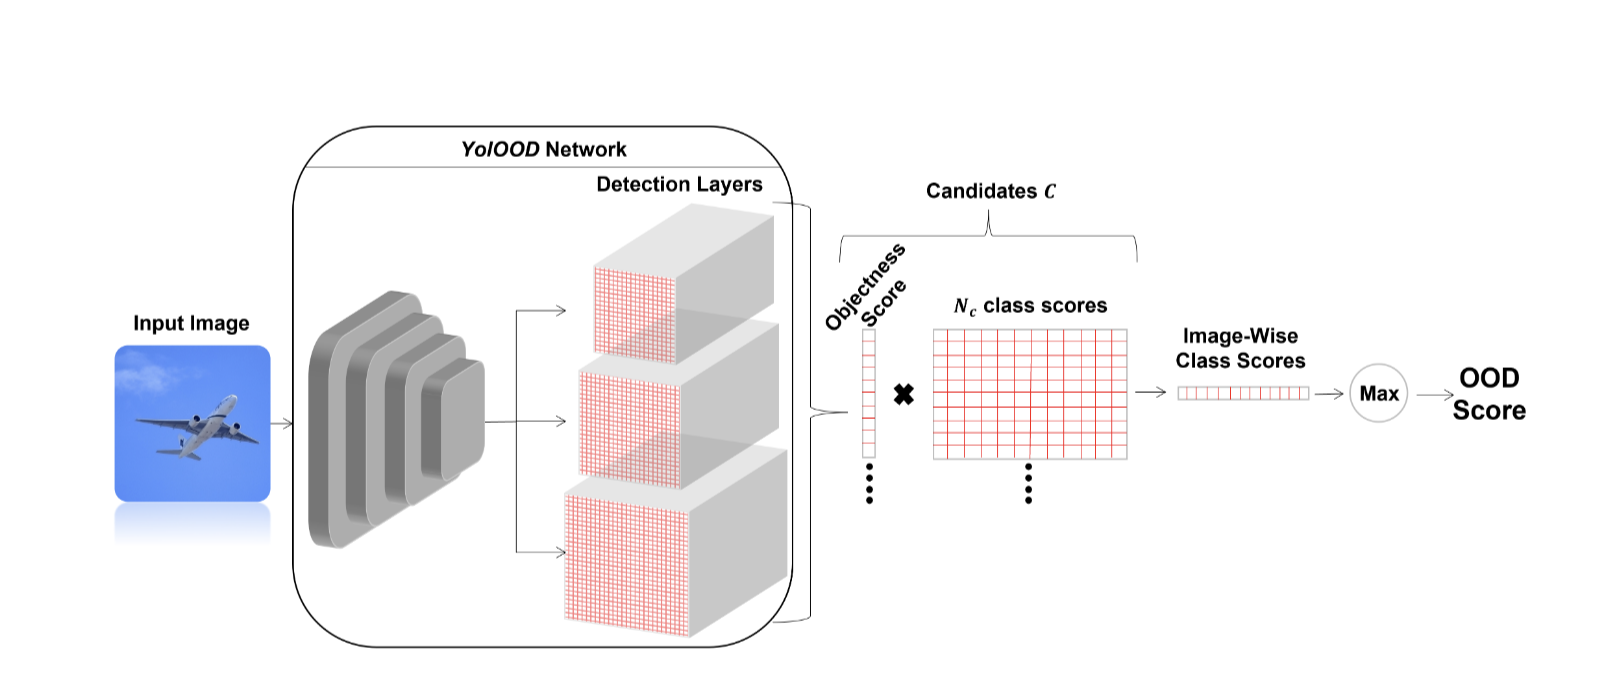
\includegraphics[width=\linewidth]{fig/yolood_arch.png}
\caption{YolOOD's pipeline.}
\label{fig:yolo}
\end{figure}
